\documentclass[../cours_3e.tex]{subfiles}
\begin{document}
\setcounter{chapter}{4}
\chapter{Calcul littéral et identités}
\label{ch:litteral}
\begin{objectif}
Traduire une situation, développer, réduire, factoriser et prouver une propriété avec des lettres. Prérequis : priorités, signes et fractions.
\end{objectif}
\section{À quoi sert une lettre ?}
Une lettre peut représenter une valeur qui varie, une inconnue à chercher ou un nombre quelconque dans une propriété. Dans $A=\pi r^2$, $r$ varie avec le disque. Dans $3x+2=11$, $x$ est inconnu. Dans $a(b+c)=ab+ac$, les lettres représentent tous les nombres auxquels la formule s'applique.
\begin{definition}
Une \textbf{expression littérale} est une expression contenant des lettres. Une \textbf{identité} est une égalité vraie pour toutes les valeurs autorisées des lettres.
\end{definition}
Les conventions abrègent la multiplication : $3\times x=3x$, $a\times b=ab$, $x\times x=x^2$ et $1x=x$. Mais $x+x=2x$ et non $x^2$.
\begin{exemple}[Substituer]
Pour $x=-2$, $3x^2-5x+1=3(-2)^2-5(-2)+1=12+10+1=23$. Mettre une valeur négative entre parenthèses évite les ambiguïtés.
\end{exemple}
\utilite{Une seule expression décrit de nombreux cas. Elle permet aussi de démontrer une propriété générale ou de programmer un calcul.}
\section{Distributivité et réduction}
\begin{propriete}
\[k(a+b)=ka+kb,\qquad k(a-b)=ka-kb.\]
\end{propriete}
La distributivité est une propriété de base des nombres, admise pour tous les réels. Pour des entiers positifs, elle découle du regroupement d'additions répétées. Pour des longueurs positives, un rectangle en donne une interprétation :
\begin{center}
\begin{tikzpicture}[scale=.75]
\draw[fill=accent!8](0,0)rectangle(7,2.2);
\draw(4,0)--(4,2.2);
\node at(2,1.1){$ka$};\node at(5.5,1.1){$kb$};
\node[left]at(0,1.1){$k$};\node[below]at(2,0){$a$};\node[below]at(5.5,0){$b$};
\end{tikzpicture}
\end{center}
La grande aire est à la fois $k(a+b)$ et $ka+kb$. Le dessin illustre la propriété pour des longueurs, mais ne suffit pas à prouver le cas des nombres négatifs.
\begin{definition}
\textbf{Développer}, c'est transformer un produit en somme. \textbf{Réduire}, c'est regrouper les termes de même nature. \textbf{Factoriser}, c'est transformer une somme en produit.
\end{definition}
On réduit $3x+5x=8x$ par distributivité : $(3+5)x=8x$. En revanche, $3x+5x^2$ contient deux types de termes.
\begin{exemple}
\[
-2(3x-4)+5(x+1)=-6x+8+5x+5=-x+13.
\]
L'opposé d'une somme change tous ses signes : $-(3x-7)=-3x+7$, car on multiplie par $-1$.
\end{exemple}
\section{Double distributivité}
\begin{propriete}
\[(a+b)(c+d)=ac+ad+bc+bd.\]
\end{propriete}
\begin{demonstration}
On distribue d'abord le facteur $(a+b)$ :
\[(a+b)(c+d)=(a+b)c+(a+b)d.\]
Puis chaque produit : $(a+b)c=ac+bc$ et $(a+b)d=ad+bd$. Réordonner donne la formule.
\end{demonstration}
\begin{exemple}
\[(2x-3)(x+4)=2x^2+8x-3x-12=2x^2+5x-12.\]
Chaque terme du premier facteur multiplie chaque terme du second. Avec deux termes dans chaque parenthèse, il y a quatre produits avant réduction.
\end{exemple}
\section{Trois identités expliquées}
\begin{propriete}
\[
(a+b)(a-b)=a^2-b^2.
\]
Compléments utiles :
\[
(a+b)^2=a^2+2ab+b^2,\qquad
(a-b)^2=a^2-2ab+b^2.
\]
\end{propriete}
\begin{demonstration}
La double distributivité donne
\[
(a+b)(a-b)=a^2-ab+ab-b^2=a^2-b^2,
\]
puis $(a+b)(a+b)=a^2+ab+ab+b^2$. Remplacer $b$ par $-b$ dans cette dernière identité donne la formule du carré d'une différence.
\end{demonstration}
L'identité de différence de carrés est explicitement attendue ; les deux autres enrichissent la compréhension et préparent le lycée.
\begin{center}
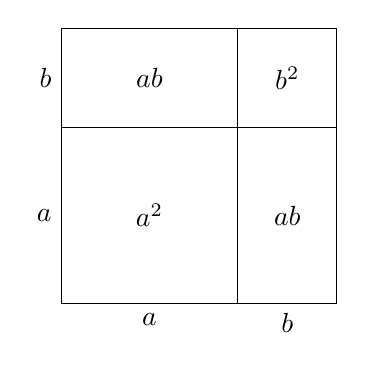
\begin{tikzpicture}[scale=.7]
\draw(0,0)rectangle(5,5);\draw(3.2,0)--(3.2,5);\draw(0,3.2)--(5,3.2);
\node at(1.6,1.6){$a^2$};\node at(4.1,1.6){$ab$};
\node at(1.6,4.1){$ab$};\node at(4.1,4.1){$b^2$};
\node[below]at(1.6,0){$a$};\node[below]at(4.1,0){$b$};
\node[left]at(0,1.6){$a$};\node[left]at(0,4.1){$b$};
\end{tikzpicture}
\end{center}
Les deux rectangles $ab$ montrent pourquoi le terme $2ab$ ne doit pas disparaître.
\begin{exemple}
$99^2=(100-1)^2=10000-200+1=9801$. De même, $103\times97=(100+3)(100-3)=10000-9=9991$.
\end{exemple}
\section{Factoriser : reconnaître le chemin inverse}
\begin{methode}
Chercher d'abord un facteur commun ; sinon reconnaître une différence de carrés. Vérifier la factorisation en redéveloppant.
\end{methode}
\begin{exemple}
\[
12x^2-18x=6x(2x-3),\qquad
9x^2-25=(3x-5)(3x+5).
\]
Le facteur commun peut être une expression :
\[
(x+2)(3x-1)+5(x+2)=(x+2)(3x+4).
\]
Et $x^2-7=(x-\sqrt7)(x+\sqrt7)$ puisque $(\sqrt7)^2=7$.
\end{exemple}
\begin{attention}
$a^2+b^2$ n'est pas une différence de carrés. Il ne faut pas inventer une factorisation de la forme $(a+b)^2$. Toutes les expressions ne se factorisent pas avec les outils de troisième.
\end{attention}
\section{Choisir la forme utile et démontrer}
La forme développée facilite souvent un calcul d'image et la comparaison de deux expressions. La forme factorisée révèle les zéros d'un produit et certains facteurs communs.
\begin{exemple}[Deux programmes identiques]
Programme A : choisir $x$, ajouter $3$, multiplier par $2$, retirer $x$. On obtient $2(x+3)-x=x+6$. Programme B : ajouter directement $6$. Les deux programmes donnent le même résultat pour tout nombre, car leurs expressions sont identiques.
\end{exemple}
\begin{demonstration}
La différence des carrés de deux entiers consécutifs est impaire :
\[(n+1)^2-n^2=n^2+2n+1-n^2=2n+1.\]
C'est la forme d'un entier impair, quel que soit l'entier $n$.
\end{demonstration}
\begin{retenir}
Développer et factoriser sont des transformations inverses. Le signe égal signifie que la valeur est conservée pour chaque valeur autorisée de la lettre. Un essai numérique détecte parfois une erreur, mais la distributivité établit l'identité.
\end{retenir}
\end{document}
